\documentclass[UTF8]{ctexart}
    \usepackage{graphicx}
    \title{HfiA Modeling Abstract and Equations}
    \author{Zhang Zhen}
\begin{document}
    \maketitle
    \section{Block-Level Mechanism}
        \subsection{HfiA Background Knowledge}
            \textit{Ref: A Cell Cycle and Nutritional Checkpoint Controlling Bacterial Surface Adhesion}

            In this paper, author describes a novel regulatory mechanism by which the C.c. bacterium integrates cell cycle and nutritional signals to control development of an adhesive envelop structure known as holdfast.

            They discovered a novel inhibitor of holdfast development. HfiA, that is regulated downstream of lovK-lovR. They also discovered a bio-synthesis related gene named HfsJ. And the suppressing mutations in HfsJ attenuate the HfsJ-HfiA interaction.

            \textbf{These results support a model in which HfiA inhibits holdfast development via direct interaction with an enzyme required for holdfast biosynthesis}

            In conclusion, author says: We demonstrate that the predicted glycosyltransferase, HfsJ, is a required component of the holdfast development machinery and that residues at the C-terminus of HsfJ mediate a direct interation with HfiA, leading to a post-translational inhibition of HfsJ.

            The binding affinity and cellular concentrations of HfiA and HfsJ are tuned such that this regulatory system is responsive to small changes rather than robust to large changes. This prediction is consistent with a highly responsive and sensitive regulatory system.

        \subsection{HfiA Modeling Abstract}
        So the block is clear. Upstream promoter Expression Rate $\rightarrow$ HfiA $\rightarrow$ HfsJ $\rightarrow$ Catalysing Rate

    \section{Equations}
    \subsection{Diagram}
            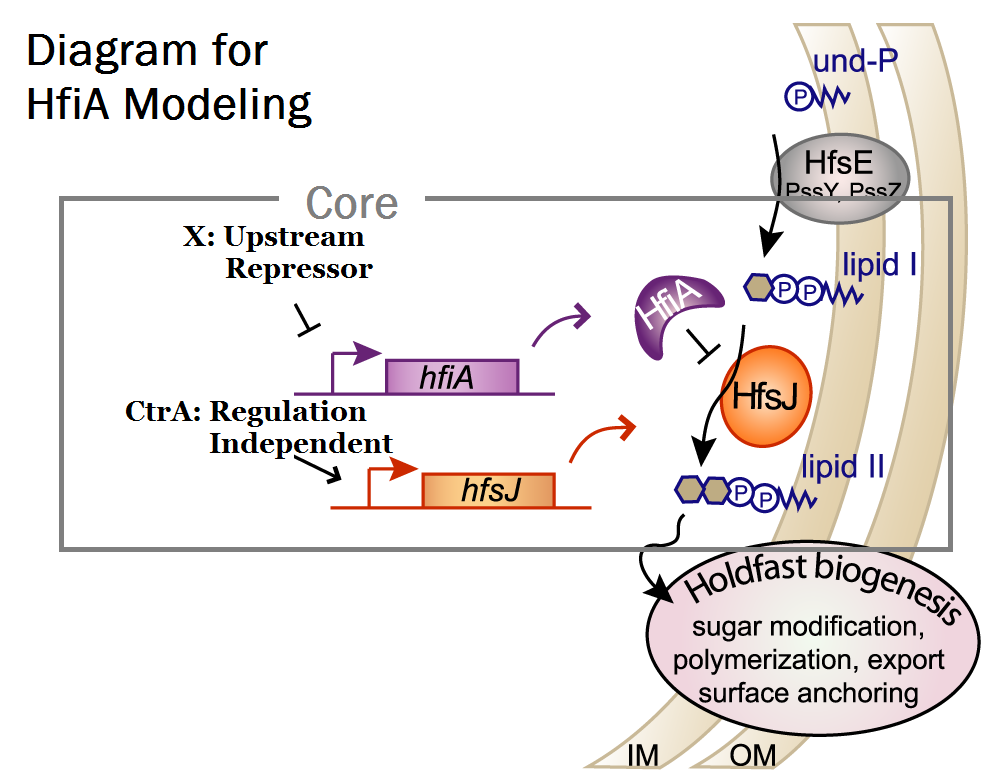
\includegraphics[width=4.00in, height=3.00in]{HfiA.png}
    \subsection{Definations:}
        \begin{enumerate}
        \item The maximum transcriptional rate of HfiA gene: $\beta_{HfiA}$
        \item The transcriptional rate of HfsJ gene: $\beta_{HfsJ}$
        \item The repressor effect: $X$
        \item The dissociation constant of repressor and HfiA: $Kd_{HfiA}$
        \item The translation rate of HfiA: $\alpha_{HfiA}$
        \item The amount of HfiA protein: $P_{HfiA}$
        \item The degradation rate of HfiA: $k_{HfiA}$
        \item The translation rate of HfsJ: $\alpha_{HfsJ}$
        \item The amount of enzyme HfsJ: $Ez_{HfsJ}$
        \item The amount of complex of HfiA and HfsJ: $C_{HfiA-HfsJ}$
        \item The dissociation constant of HfiA-HfsJ: $Kd_{C_{HfiA-HfsJ}}$
        \item The degradation rate of HfsJ: $k_{HfsJ}$
        \item The amount of valid enzyme HfsJ: : $Ez^{*}_{HfsJ}$
        \end{enumerate}
    \section{Equations:}
        \begin{enumerate}
        \item Actual transcriptional rate of HfiA: $$\beta_{HfiA}^{*} = \frac{\beta_{HfiA}}{1+\frac{X}{Kd_{HfiA}}}$$
        \item  The changing rate of HfiA amount: $$\frac{dP_{HfiA}}{dt} = \beta_{HfiA}\alpha_{HfiA} - k_{HfiA}P_{HfiA}$$
        \item  The changing rate of total amount of enzyme HfsJ: $$\frac{dEz_{HfsJ}}{dt}= \beta_{HfsJ}\alpha_{HfsJ} -  k_{HfsJ}Ez_{HfsJ}$$
        \item  The relationship between valid enzyme amount and total amount: $$Ez^{*}_{HfsJ} = Ez_{HsfJ}-C_{HfiA-HfsJ} = Ez_{HfsJ} - Kd_{C_{HfiA-HfsJ}}P_{HfiA}Ez_{HfsJ}$$
        \item  The output function: $$Adhesion = f(Ez^{*}_{HfsJ})$$
        \end{enumerate}

\end{document} 